% 1. Introduction
% - Motivation [understandable also for a general audience]
% - Problem statement [formulation of research question]
% (- Own contributions [novelties you claim as your own])
% (- Organization of thesis [brief description of how the remaining chapters are organized])


\section{Motivation}\label{sec:motivation}
\label{motivation}

\Gls{sv} is a biometric process used to verify the identity of a speaker based on their voice characteristics. It differs from \gls{si}, which involves identifying a speaker among a group. In \gls{sv}, the system compares the incoming speech data against another speech recording of a claimed identity to confirm whether the claim is true. Essentially, the task is binary - confirming or denying the identity claim - making it particularly suitable for access control and authentication purposes. \Gls{sv} and \gls{si} are subtasks of the broader field \gls{sr} \cite{kinnunen2006realtime}. Figure \ref{fig:difference_sv_si} shows the difference between the two tasks.

\begin{figure}[h]
    \centering
    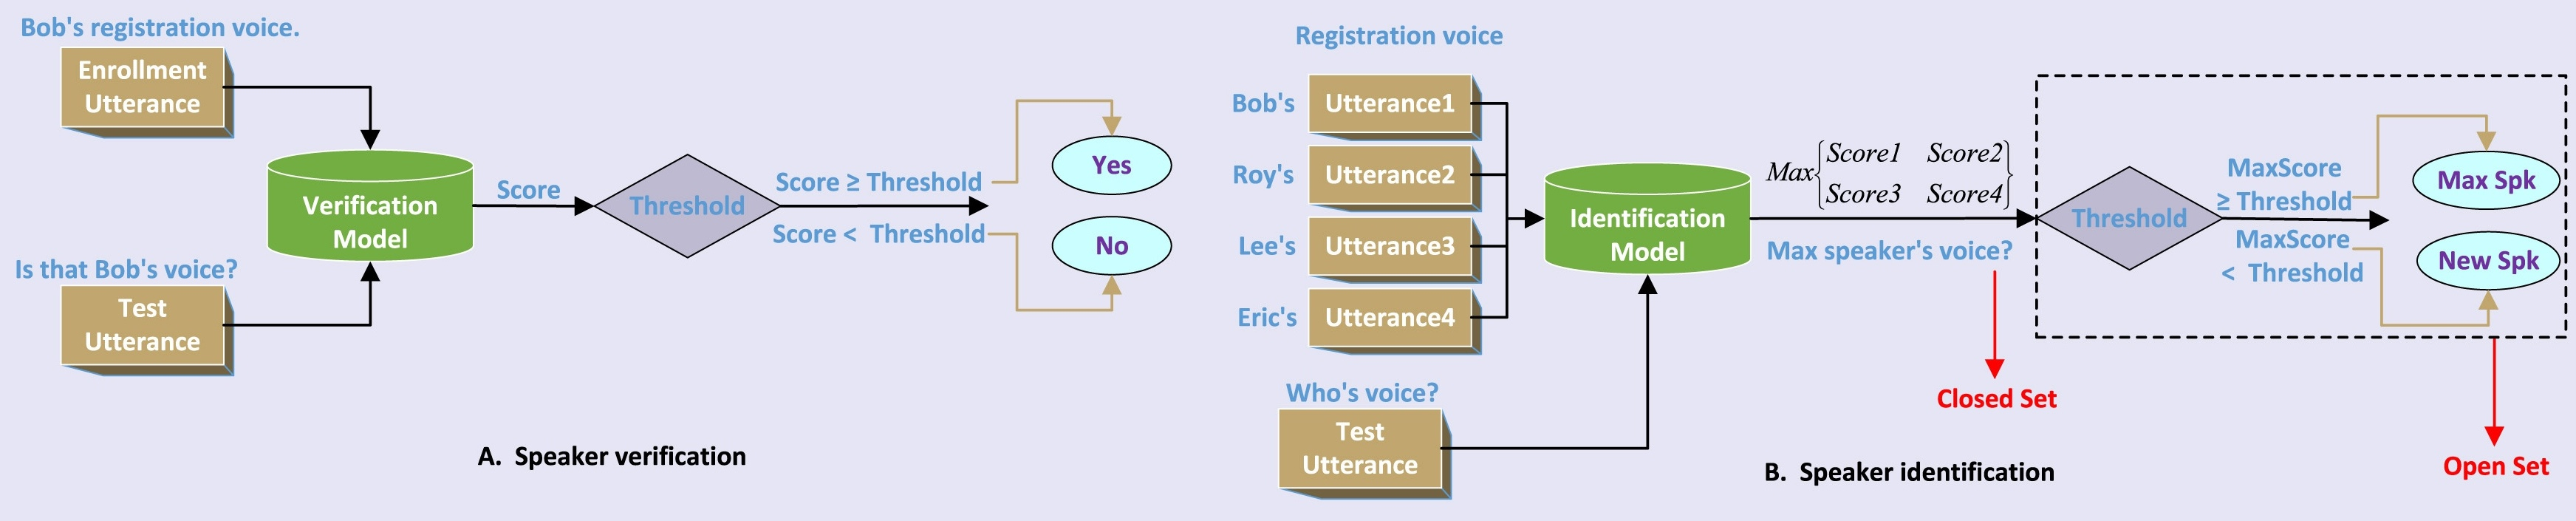
\includegraphics[width=\textwidth]{img/speaker_identification_verification.jpg}
    \caption{Difference between speaker verification and identification. Image from \cite{bai2021speaker}.}
    \label{fig:difference_sv_si}
\end{figure}

With the proliferation of smart devices and voice-activated interfaces such as Siri, Cortana, and Alexa, \gls{sv} has become an indispensable technology in ensuring secure and personalized user experiences. These systems rely on the unique characteristics of a user's voice to confirm their identity, enabling tasks ranging from sending messages to making purchases. Despite significant advancements, automatic \gls{sv} systems still face challenges, particularly in noisy or unpredictable environments, where they often struggle to maintain accuracy and reliability \cites{khazaleh2024investigation, sun2023noise}.

Humans excel in recognizing speakers even in adverse conditions, a skill partly attributable to their adeptness at interpreting prosodic features - subtle variations in rhythm, stress, and intonation that convey important information about the speaker's identity \cites{rose2002forensic, hansen2015speaker}. Similarly, enhancing the capability of machines to understand and utilize these prosodic cues could markedly improve \gls{sv} systems, especially in challenging scenarios \cite{stadelmann2009unfolding}. Henceforth, we refer to this type of information as \gls{sst}, which is distinguished from \gls{fba}, referring to short-term spectral information. % fba is short-term spectral information only in machines? 

\Glspl{dnn} have become very good at \gls{sv} \cite{huh2023voxsrc}. It was therefore often assumed that, similar to humans, they are now able to make use of \gls{sst} as well \cites{stadelmann2018capturing, zhao2020improving, ye2021deep}. However, recent research shows that at least for some architectures, such as \glspl{cnn}, \glspl{rnn}, and \glspl{resnet} this hypothesis needs to be rejected. Specifically it was found that for the aforementioned models, when trained on manipulated data that does not contain any \gls{sst} anymore, the performance does not decrease as expected, but stays the same or sometimes even increases \cite{neururer2023deep}. This "\textit{deep cheating}" phenomenon is significant as it suggests a potential path to improving the performance, reliability and robustness of \gls{sv} systems.

This leads us to question whether a different architectural approach could surmount these obstacles. Consequently, this thesis proposes the exploration of transformers \cite{vaswani2017attention}, renowned for their effectiveness in sequence-based tasks and potential for modeling complex dependencies over time. By investigating these models' ability to utilize \gls{sst}, we aim to uncover whether they can enhance the accuracy and robustness of \gls{sv} systems.


\section{Problem Statement}

This thesis aims to investigate the modeling of \gls{sst} in transformer models, a type of neural network architecture for example associated with \glspl{llm} like ChatGPT. By pre-training these models to reconstruct hidden frames in speech spectrograms, it is hypothesized that they can better capture the temporal nuances of speech, leading to improved \gls{sv} accuracy, overall through enhanced capturing of supra-segmental features.

To test these assertions, experiments are conducted with transformers focusing on the capture of \gls{sst}. Performance comparisons are made between models trained on original speech data and those trained on manipulated data devoid of any temporal information. The outcomes of these experiments will help assess the efficacy of transformers in \gls{sv} tasks and their ability to robustly model essential speech characteristics.


\section{Contributions}

While not achieving state-of-the-art, we can show that for the transformer architecture (at least when using the configuration described in chapter \ref{chapter:methods}) the same oddity holds true as for the other architectures tested in \cite{neururer2023deep}. Specifically, training with data that includes \gls{sst} does not improve \gls{sv} performance; on the contrary, it actually has a detrimental impact on the latter.


\section{Organization}\label{sec:organization}

The rest of this thesis is organized into four chapters and two appendices:

\begin{itemize}
    \item \textbf{Chapter \ref{chapter:foundation}: Foundations} covers foundational concepts related to \gls{sv} on a high level. It also reviews the related work this thesis builds upon.
    \item \textbf{Chapter \ref{chapter:methods}: Methods} contains a detailed description of the methodologies employed in this thesis, focusing on data preprocessing as well as pretraining and finetuning of the model.
    \item \textbf{Chapter \ref{chapter:results}: Results} presents the results of the conducted experiments as well as a discussion thereof. The pretraining results are presented and the tendency of transformers, when finetuned for \gls{sv}, to model \gls{sst} is discussed.
    \item \textbf{Chapter \ref{chapter:conclusion}: Conclusion} summarizes the findings of the thesis and discusses their implications for future research in \gls{sv}.
    \item \textbf{Appendix \ref{appendix_resynth}: Resynthesizing Audio from Spectrograms} describes a problem we encountered when resynthesizing audio from spectrograms and the solution we came up with to mitigate it.
    \item \textbf{Appendix \ref{appendix_resynth_examples}: More Resynthesized Spectrograms} contains additional resynthesized spectrograms that were developed during our project.
\end{itemize}
\pagebreak [3]


\section{Implementation}\label{sec:implementation}
The code developed for this project is publicly available at the following URL:\\ \href{https://github.com/Ironmomo/SpeakerVerificationBA}{https://github.com/Ironmomo/SpeakerVerificationBA}.
























% In recent years, advancements in automatic speaker recognition technology have been notable, mainly due to the development of deep learning methods \cite{brown2022voxsrc, huh2023voxsrc}. However, these systems still struggle to match human performance, especially in challenging conditions like background noise or with short utterances from unknown speakers. Research at \gls{zhaw} has identified a significant gap in how \glspl{dnn} comprehend and use speaker-specific traits such as \gls{sst} in \gls{sr} \cite{neururer2023deep}.

% Existing literature emphasizes the importance of speaker-specific traits and the ability of \glspl{dnn} to learn them. Yet, studies show that current \glspl{cnn}, \glspl{rnn}, and \glspl{resnet} used for \gls{sv} and \gls{sc} often overlook these traits when trained on clean datasets. This phenomenon, termed "\textit{deep cheating}" is significant as it suggests a potential path to improving related tasks and reducing error rates.




% The objectives of the thesis include:
% \begin{itemize}

% \item Conducting a thorough review of relevant literature and previous studies to identify existing approaches and gaps in research.
% \item Collaboratively devising a clear approach, guided by supervisors, including defining the architecture and training methods for transformer models.
% \item Setting up the necessary infrastructure for data collection and processing, including local setups and GPU resources.
% \item Developing and refining a prototype of the transformer-based speaker recognition system through innovative experimentation.
% \item Ultimately, presenting a scholarly document outlining the motivation, methodology, evaluations, and findings of the research, emphasizing the advancements in speaker recognition achieved through transformer models.
% \end{itemize}

% This thesis aims to contribute meaningfully to the ongoing discussion on voice recognition while addressing the current limitations of automatic speaker recognition systems.















